% Options for packages loaded elsewhere
\PassOptionsToPackage{unicode}{hyperref}
\PassOptionsToPackage{hyphens}{url}
%
\documentclass[
  12pt,
  a5paper,
  twoside]{book}

\usepackage{amsmath,amssymb}
\usepackage{iftex}
\ifPDFTeX
  \usepackage[T1]{fontenc}
  \usepackage[utf8]{inputenc}
  \usepackage{textcomp} % provide euro and other symbols
\else % if luatex or xetex
  \usepackage{unicode-math}
  \defaultfontfeatures{Scale=MatchLowercase}
  \defaultfontfeatures[\rmfamily]{Ligatures=TeX,Scale=1}
\fi
\usepackage{lmodern}
\ifPDFTeX\else  
    % xetex/luatex font selection
    \setmainfont[]{Times New Roman}
\fi
% Use upquote if available, for straight quotes in verbatim environments
\IfFileExists{upquote.sty}{\usepackage{upquote}}{}
\IfFileExists{microtype.sty}{% use microtype if available
  \usepackage[]{microtype}
  \UseMicrotypeSet[protrusion]{basicmath} % disable protrusion for tt fonts
}{}
\makeatletter
\@ifundefined{KOMAClassName}{% if non-KOMA class
  \IfFileExists{parskip.sty}{%
    \usepackage{parskip}
  }{% else
    \setlength{\parindent}{0pt}
    \setlength{\parskip}{6pt plus 2pt minus 1pt}}
}{% if KOMA class
  \KOMAoptions{parskip=half}}
\makeatother
\usepackage{xcolor}
\usepackage[inner=0.8in,outer=0.5in,top=0.9in,bottom=0.9in]{geometry}
\setlength{\emergencystretch}{3em} % prevent overfull lines
\setcounter{secnumdepth}{5}
% Make \paragraph and \subparagraph free-standing
\makeatletter
\ifx\paragraph\undefined\else
  \let\oldparagraph\paragraph
  \renewcommand{\paragraph}{
    \@ifstar
      \xxxParagraphStar
      \xxxParagraphNoStar
  }
  \newcommand{\xxxParagraphStar}[1]{\oldparagraph*{#1}\mbox{}}
  \newcommand{\xxxParagraphNoStar}[1]{\oldparagraph{#1}\mbox{}}
\fi
\ifx\subparagraph\undefined\else
  \let\oldsubparagraph\subparagraph
  \renewcommand{\subparagraph}{
    \@ifstar
      \xxxSubParagraphStar
      \xxxSubParagraphNoStar
  }
  \newcommand{\xxxSubParagraphStar}[1]{\oldsubparagraph*{#1}\mbox{}}
  \newcommand{\xxxSubParagraphNoStar}[1]{\oldsubparagraph{#1}\mbox{}}
\fi
\makeatother


\providecommand{\tightlist}{%
  \setlength{\itemsep}{0pt}\setlength{\parskip}{0pt}}\usepackage{longtable,booktabs,array}
\usepackage{calc} % for calculating minipage widths
% Correct order of tables after \paragraph or \subparagraph
\usepackage{etoolbox}
\makeatletter
\patchcmd\longtable{\par}{\if@noskipsec\mbox{}\fi\par}{}{}
\makeatother
% Allow footnotes in longtable head/foot
\IfFileExists{footnotehyper.sty}{\usepackage{footnotehyper}}{\usepackage{footnote}}
\makesavenoteenv{longtable}
\usepackage{graphicx}
\makeatletter
\newsavebox\pandoc@box
\newcommand*\pandocbounded[1]{% scales image to fit in text height/width
  \sbox\pandoc@box{#1}%
  \Gscale@div\@tempa{\textheight}{\dimexpr\ht\pandoc@box+\dp\pandoc@box\relax}%
  \Gscale@div\@tempb{\linewidth}{\wd\pandoc@box}%
  \ifdim\@tempb\p@<\@tempa\p@\let\@tempa\@tempb\fi% select the smaller of both
  \ifdim\@tempa\p@<\p@\scalebox{\@tempa}{\usebox\pandoc@box}%
  \else\usebox{\pandoc@box}%
  \fi%
}
% Set default figure placement to htbp
\def\fps@figure{htbp}
\makeatother

% Shared LaTeX styling for book projects
% Save as: island-tales-shared-book-style.tex

% Document initialization (equivalent to your \AtBeginDocument block)
\usepackage{fncychap}
\usepackage{geometry}
\AtBeginDocument{
  \date{}
  \setcounter{tocdepth}{0}
  \setcounter{secnumdepth}{0}
  %\newgeometry{twoside,inner=0.9in,outer=0.5in,top=1in,bottom=1in}
  
  % The \headsep sets the distance between header line and body text
  \setlength{\headsep}{16pt}

  \clubpenalty=10000
  \widowpenalty=100000
  \displaywidowpenalty=10000
  \tolerance=1000
  \hyphenpenalty=50
  \exhyphenpenalty=50

  \let\origtableofcontents\tableofcontents
  \renewcommand{\tableofcontents}{%
    \cleardoublepage
    \pagestyle{plain}
    \origtableofcontents
    \cleardoublepage
    \pagestyle{normal} 
  }
}

% Chapter formatting
\usepackage{titlesec}
\titleformat{\chapter}[display]
  {\normalfont\huge\bfseries\hyphenpenalty=10000\exhyphenpenalty=10000}
  {}
  {0pt}
  {\Huge}
\titlespacing*{\chapter}{0pt}{-10pt}{20pt}

% Code font size (Sphinx compatibility)
%\renewcommand{\sphinxcode}[1]{\texttt{\footnotesize #1}}
%\renewcommand{\sphinxupquote}[1]{#1}
\let\oldtexttt\texttt        % save original \texttt
\renewcommand{\texttt}[1]{{\footnotesize\oldtexttt{#1}}}

% Custom page styles with fancyhdr
\usepackage{fancyhdr}
\makeatletter
\fancypagestyle{normal}{
    \fancyhf{}
    \fancyhead[RE]{{\small\textit{\@title}}}
    \fancyhead[LO]{{\small\nouppercase{\textit{\leftmark}}}}
    \fancyhead[LE]{{\small\thepage}}
    \fancyhead[RO]{{\small\thepage}}
    \fancyfoot[LE,LO,RE,RO]{}
    \setlength{\footskip}{0pt}
    \addtolength{\textheight}{20pt}
    \renewcommand{\headrulewidth}{0.4pt}
}
\makeatother


\fancypagestyle{plain}{
    % first page of new chapter
    \fancyhf{}
    \fancyfoot[LE,LO,RE,RO]{}
    \setlength{\footskip}{0pt}
    \addtolength{\textheight}{20pt}
    \renewcommand{\headrulewidth}{0pt}
}

% New header
%\usepackage{titling}
\usepackage{hyperref}
\newfontfamily\headingfont[]{Gill Sans}


\makeatletter
\renewcommand{\maketitle}{%
  \thispagestyle{plain}
  \noindent\rule{\linewidth}{1pt}\par
  \begingroup
    \hypersetup{pdfauthor={\@author}, pdftitle={\@title}}%
  \endgroup
  \begin{flushright}
    \vspace{48pt}
    {\headingfont
    {\fontsize{44pt}{56pt}\selectfont \setlength{\baselineskip}{56pt}%
    \@title\par}
    \vspace{96pt}
    % HACK to handle quote
    %{\Large \@author}\par
    {\Large Tony {\textquotesingle}Monty{\textquotesingle} Hirst}\par
    
    \vspace{25pt}
    \@date \par

    }
  \end{flushright}

  
  \newpage
  \thispagestyle{plain}
  \thispagestyle{empty}

  \makeatletter

  \vspace*{\fill}

  \begin{center}
  %{\Large \textbf{\@title}}\\[1em]
  {\large \textbf{\textit{A Storynotes Collection}}}\\[2em]
  \end{center}

  \vfill

  \begin{center}
  \large \textit{montystoryteller.org}
  \end{center}

  \vspace{2cm}

  \begin{center}
  \textit{Copyright {\copyright} Anthony Hirst, 2025.\linebreak\linebreak This work may include transcripts of nineteenth century newspaper articles contemporary to the events described, sourced from the British Newspaper Archive, and transcribed by the author.\linebreak\linebreak This work may include transcripts of out of copyright works published prior to 1920 sourced from the Internet Archive.\linebreak\linebreak This work may include other openly licensed materials, acknowledged at the point of use.
  }
  \end{center}

  \vspace*{\fill}

  \begin{center}
    \textit{A Storynotes publication from montystoryteller.org}
  \end{center}
  \makeatother

  \setcounter{footnote}{0}
  \let\thanks\relax\let\maketitle\relax
}
\makeatother

\renewcommand{\chaptermark}[1]{%
  \markboth{#1}{}}

\usepackage{caption}
\captionsetup[figure]{labelformat=empty}

% Apply normal page style (equivalent to fancy in Quarto)
\pagestyle{normal}
\makeatletter
\@ifpackageloaded{bookmark}{}{\usepackage{bookmark}}
\makeatother
\makeatletter
\@ifpackageloaded{caption}{}{\usepackage{caption}}
\AtBeginDocument{%
\ifdefined\contentsname
  \renewcommand*\contentsname{Table of contents}
\else
  \newcommand\contentsname{Table of contents}
\fi
\ifdefined\listfigurename
  \renewcommand*\listfigurename{List of Figures}
\else
  \newcommand\listfigurename{List of Figures}
\fi
\ifdefined\listtablename
  \renewcommand*\listtablename{List of Tables}
\else
  \newcommand\listtablename{List of Tables}
\fi
\ifdefined\figurename
  \renewcommand*\figurename{Figure}
\else
  \newcommand\figurename{Figure}
\fi
\ifdefined\tablename
  \renewcommand*\tablename{Table}
\else
  \newcommand\tablename{Table}
\fi
}
\@ifpackageloaded{float}{}{\usepackage{float}}
\floatstyle{ruled}
\@ifundefined{c@chapter}{\newfloat{codelisting}{h}{lop}}{\newfloat{codelisting}{h}{lop}[chapter]}
\floatname{codelisting}{Listing}
\newcommand*\listoflistings{\listof{codelisting}{List of Listings}}
\makeatother
\makeatletter
\makeatother
\makeatletter
\@ifpackageloaded{caption}{}{\usepackage{caption}}
\@ifpackageloaded{subcaption}{}{\usepackage{subcaption}}
\makeatother

\usepackage{bookmark}

\IfFileExists{xurl.sty}{\usepackage{xurl}}{} % add URL line breaks if available
\urlstyle{same} % disable monospaced font for URLs
\hypersetup{
  pdftitle={A Legend of Puckaster Cove},
  pdfauthor={Tony `Monty' Hirst},
  hidelinks,
  pdfcreator={LaTeX via pandoc}}


\title{A Legend of Puckaster Cove}
\author{Tony `Monty' Hirst}
\date{}

\begin{document}
\frontmatter
\maketitle

\renewcommand*\contentsname{Contents}
{
\setcounter{tocdepth}{0}
\tableofcontents
}

\mainmatter
\bookmarksetup{startatroot}

\chapter{Preface}\label{preface}

What's in a name?

John Whitehead's \emph{The Undercliff of the Isle of Wight} (1911) cites
volume II of Roach Smith's \emph{Retrospections, Social and
Archaeological}, of 1886, as follows:

\begin{quote}
\emph{``Puck, Pixies, and Fairies, have left numerous records of their
influence over public credulity, and the places named from them are
usually associated with remains of antiquity of some kind. Puckaster, or
Puckaster Cove, at the back of the Isle of Wight, is one of the
localities which has attracted the attention of several writers, and
some have been led to imagining that it is of Roman origin. A short time
since I had an excellent opportunity of surveying Puckaster. As I
approached the site I could see from landslips in remote times the
dislocated masses had taken a fantastic form, something like that of a
castle or fortified place, and to Puck it had consequently been
assigned.''}
\end{quote}

According to A. D. Mills' \emph{The Place-names of the Isle of Wight},
the name of Puckaster Cove derives not from the Latin \emph{Port
Castra}, but is more likely derived from the Old English words
\emph{puca} (from which we get puck), and \emph{torr}, which together
give us \emph{``the rock or rocky hill haunted by a goblin''}.

Mills also suggests that the nearby Puckwell Farm, apparently recorded
in 1461 as \emph{Pokewell}, derives in part from the Old English
\emph{wella}, to give us \emph{``the string or stream haunted by a
goblin''}.

If we are to go in search of fairy stories from the Isle of Wight, then
--- \emph{real} fairy stories --- we should, perhaps, start by looking
for tales set around the location of Puckaster Cove.

And we should also consult the ``honourable'' Mr.~Abraham Elder, teller
of fantastic tales and legends about the Isle of Wight. Consulting the
first edition of his book of that same name, \emph{Tales and Legends of
the Isle of Wight}, published in 1839, we see no reference to any legend
of Puckaster Cove, although it does appear in the second edition of 1843
(a copy of this work can be viewed \emph{by appointment} in the Caste
Museum library collection at Carisbrooke Castle). The story can also be
found in the pages of \emph{Bentley's Miscellany}, a nineteenth literary
magazine published under the editorship of a certain Mr Charles Dickens.

Here, then, is that tale re-published, along with my own version of it,
originally told as part of the \emph{'Tis Tales} storytelling set,
\emph{Island Tales} at Ventnor Fringe, 2022.

--Tony ``Monty'' Hirst\\
Apse Heath, September 2022.

\let\thefootnote\relax\footnotetext{To keep up to date with traditional storytelling events and activities on the Isle of Wight, make sure you check the `Tis Tales website — tistales.org.uk — regularly. For more storynotes publications, please visit montystoryteller.org}

\begin{figure}[H]

{\centering 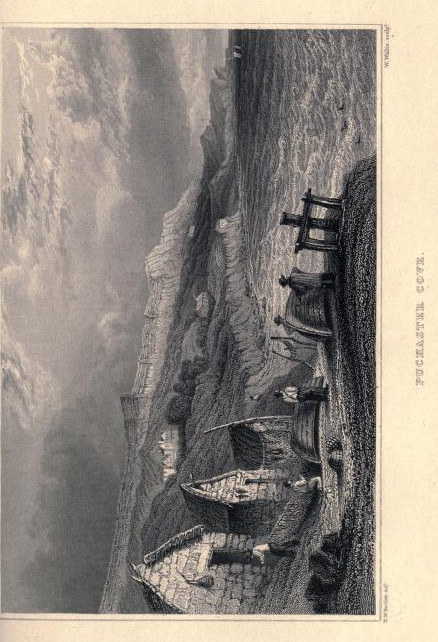
\includegraphics[width=0.75\linewidth,height=\textheight,keepaspectratio]{images/barberspicturesq00barbiala_0191-cropped.jpg}

}

\caption{Puckaster Cove, in Barber's Picturesque}

\end{figure}%

\emph{Puckaster Cove, in Barber's picturesque illustrations, of the Isle
of Wight, comprising views of every object of interest on the island,
1834.}

\bookmarksetup{startatroot}

\chapter{A Legend of Puckaster}\label{a-legend-of-puckaster}

\textbf{\emph{As originally told by Abraham Elder, ``A Legend of
Puckaster'', in Bentley's Miscellany,
\href{https://archive.org/details/sim_bentleys-miscellany_1839-07_6/page/368/mode/2up}{volume
5}, 1839. The footnotes also appeared in the original version.}}

A LEGEND OF PUCKASTER,\\
ISLE OF WIGHT.\\
BY ABRAHAM ELDER, ESQ.

John Kann was a labouring man, living in the parish of Whitewell; and,
in the good old times, when fairies danced, was said to have been
particularly favoured by them. This was a matter of considerable
importance at the time, for he lived in a neighbourhood where they were
most numerous and active.
\texttt{{[}Burton,\ in\ his\ Anatomy\ of\ Melancholy,\ tells\ us\ that\ "terrestrial\ devils\ are\ those\ lares,\ genii,\ fauns,\ satyrs,\ wood-nymphs,\ foliots,\ fairies,\ Robin\ Goodfellows,\ trulli,\ \&c.\ which,\ as\ they\ are\ most\ conversant\ with\ men,\ so\ they\ do\ them\ much\ harm.\ These\ are\ they\ that\ dance\ on\ heaths\ and\ greens,\ as\ Lavater\ thinks\ with\ Trithemius,\ and\ as\ Olaus\ Magnus\ adds,\ leave\ that\ green\ circle\ which\ we\ commonly\ find\ in\ plain\ fields.\ They\ are\ sometimes\ seen\ by\ old\ women\ and\ children.\ Hieron.\ Pauli,\ in\ his\ description\ of\ the\ city\ of\ Bercino,\ in\ Spain,\ relates\ how\ they\ have\ been\ familiarly\ seen\ near\ that\ town,\ about\ fountains\ and\ hills.\ "Sometimes,"\ saith\ Trithemius,\ "they\ lead\ simple\ people\ into\ the\ recesses\ of\ the\ mountains,\ and\ shew\ them\ wonderful\ sights,\ \&.c."\ Giraldus\ Cambrensis\ gives\ instance\ of\ a\ monk\ of\ Wales\ that\ was\ so\ deluded.\ Paracelsus\ reckons\ up\ many\ places\ in\ Germany\ where\ they\ do\ usually\ walk\ about\ in\ little\ coats,\ some\ two\ feet\ long.\ —\ See\ Anatomy\ of\ Melancholy,\ 15th\ ed.\ p.\ 124.{]}}

Mr.~Puck himself, as it was very well known at the time, used frequently
to hold his court, and lead his midnight revels on a spot by the
sea-side not above a mile from his house. It was a wild uncultivated
place, covered with rocks, and bogs, and holes, and briers. It was
generally known when he was at home by a small light being seen dancing
about at midnight over the rough ground. This the neighbours used to
call ``Friar Rush's lantern,'' or ``Puck's little star'': the latter
name, however, was the most common.

Amidst all this wilderness of rocks, bogs, and briers, there was,
however, one place where the turf was extremely smooth and level; and
persons passing that way by daylight used to observe those circular
marks in the grass, which are everywhere known by the name of fairy
rings.

One day a neighbour of John Kann's said to him, ``John, I am going to
build myself a house. Come, and I will show you where. It is the
prettiest loveliest spot that ever was seen?''

Where do you think he took him to? To the very place where the grass was
so smooth and soft, and where the fairy rings were always seen.

``Gracious me!'' said John Kann. ``You are not going to build here! Are
you not afraid of Puck's little star? By St.~Radegund you are making a
fool of me!''
\texttt{{[}St.\ Radegund\ appears\ to\ have\ been\ the\ patroness\ saint\ of\ Whitewell.\ There\ was\ anciently\ a\ chapel\ dedicated\ to\ her\ there.{]}}

``I'm not making a fool of you at all,'' said he, ``but, the fact is,
now that I am going to be married, I must get a house of my own to live
in; besides, this would be a nice healthy place for the children when
they come.''

``But ain't you afraid of Puck?''

``Not at all,'' he answered. ``Puck never hurts an honest industrious
fellow like me. We have always been very good friends, and I have no
doubt but that we shall continue so.''

``And whom do you suppose the land belongs to?'' asked John Kann.

``Why, it's just waste land, and is of no use to anybody; and the manor
belongs to the Lisle family. They would never grudge a poor man's
building a cottage there.''

``That spot,'' said John Kann, ``no more belongs to the Lisles than it
belongs to me. It belongs to Mr.~Puck; and, you think it would be a nice
place for your children, do you? Do you know what happens to children
that are born on fairy ground?''

``No.''

``Why, then, I will just tell you. The fairies give them gin to prevent
them growing any bigger, and then carry them off, and put an old wizen
fairy in their place. I have known the thing happen often and often
before. That child of Sukey Grundle's, you know, that was always crying
and squealing, that was never her child at all, but just an old fairy.
Her own little darling is no doubt at this moment doing the dirty work
for some of the queer creatures in Fairy-land, scrubbing, and dusting,
and slaving, and feeding their pigs, and, no doubt, getting a whop on
the head every now and then with a broomstick; and, I will tell you
what; it's of no use your settling here, just for the purpose of
providing for your family by getting your children apprenticed out to
the fairies. It's no saving at all, for they always leave one of their
own sort, that eats twice as much, and is, besides, very mischievous, in
its place. You had better not interfere with Puck's little star.''

Well, John Kann's neighbour took his advice; and, moreover, asked John
to his wedding-feast, which took place a day or two afterwards. John
passed a very merry evening; and it was late and very dark before he
started to return home. There were no roads in this part of the island
in those days, so finding one's way home at night was not always an easy
matter. Luckily, however, for John, a friend of his, who lived near, had
started just before with a lantern, and John followed the light, which
was some way on before him, singing to himself as he went along.

Up-hill and down-hill, over rough and smooth, John Kann followed the
light: but, somehow or other he did not recognise any part of the road
as he went along. ``Maybe the ale was strong, and I am a little fuddled
like, though I do not feel so,'' thought he to himself. ``Maybe, all
this time I have been following a wrong person with a lantern.''
However, it was of no use stopping then, as he did not at all know where
he was; so he followed on, and on, and on. The ground grew rougher,
sometimes up-hill, sometimes downhill, amongst brambles, and rocks, and
holes, but there was a firm good path under his feet all the while.
When, all of a sudden a new idea flashed across his mind. ``Maybe it's
Puck's little star that I have been walking after all this while. What
fun!'' thought he to himself.

At length the light seemed to stand still, and John Kann walked up to
it. However, as he came nearer, the light seemed to grow paler and
smaller; and, when he got close to it, it was no bigger or brighter than
a glow-worm's tail, so he was left all in the dark; but just then the
moon glided out from behind a cloud, and showed him that he was on the
very spot where the grass was smooth, and the fairy rings were, and
where his neighbour wanted to have built his house.

As he stood still he thought he heard the sound of music, and a
multitude of tiny voices singing together in chorus. He held his breath,
and listened. He could clearly distinguish the following words,

``John Kann--- John Kann\\
Is a very nice man:\\
He's a very nice man,\\
John Kann.''

He looked about for some time to see whence the voices came. At length
he saw down on the ground just before him a great number of very small
little people dancing hand in hand round a ring, with red and purple
caps upon their heads, and little petticoats and cloaks, that looked as
if they were made of gossamer. They all looked so faint in the moonlight
that he thought at first it had only been the moon shining upon the
stalks of grass as they waved in the wind. How lucky it was that he had
heard them singing, or he might have walked on, and trod upon half a
dozen of them.

While he stood there, looking at the dance, there came up to him one
that looked like a very wee child of about five years of age, but his
face seemed full of fun and mischief. As he came up to John all the
fairies left off dancing, and stood hand in hand in a half circle round,
bowing and courtesying to him, saying,

``Mr.~Puck --- Mr.~Puck,\\
Give John good luck.\\
He's come to see\\
The revelry\\
On the fairy lea,\\
And to dance on his toe,\\
As round we go.\\
As round we go.''

``I don't see how I can manage to dance with you,'' said John, ``without
treading upon a good many of you, and crushing you to pieces; for you
see I am at least twice as big as all of you put together.''

Here little Master Puck put in his word.

``John Kann --- John Kann,\\
You great big man,\\
Though broad and tall.\\
We'll make you small,\\
If you'll dance with me\\
On the fairy lea.\\
There's dust on the fern ---\\
The lady's fern,\\
That waves o'er the burn.\\
Brown stripes are seen\\
On its leaves of green.\\
Go. Fetch.''

Upon which six little fairies flew away; for they had all a sort of
butterfly wings growing out from behind their shoulders, which John Kann
had not observed before. After a short time they returned, each bringing
in his hand a small acorn-cup full of a brown powder, looking very like
snuff. Mr.~Puck took a pinch of it; and, walking up to John Kann, said,

``Now --- now\\
I'll shew you how\\
We make the tall\\
Grow small. Sit down\\
Upon the groun'\\
John Kann,\\
You tall man.''

John Kann nodded assent, and squatted himself upon the turf without more
ado. Puck immediately climbed up on his knee, and then reaching up as
high as he could, he caught hold of the lowest button of John's
waistcoat, and then scrambled up a little higher. At length he got one
of his feet firmly planted upon the edge of his waistcoat-pocket, and
resting the other upon one of his buttons, he said,

``Stoop, Mr.~Kann,\\
You tall man.''

John bowed his head as he was directed, and Puck immediately crammed
some of the dust up his nostrils. John Kann gave a loud sneeze, so
violent, indeed, that it shook his hat clean off his head, to John's
great dismay, for he thought he must have crushed to death at least a
dozen of his little friends. However, they all got out of the way
quicker than thought; and, standing in a wide circle round him, they set
up a loud shout the moment they heard him sneeze, and kept on cheering
for some time. But, what was the most wonderful part of the whole, it
seemed to him that the moment he sneezed he grew considerably smaller,
shorter, and thinner; yet, as his clothes fitted him just as close, they
must have grown smaller at the same time.

Mr.~Puck administered another pinch of the powder. John Kann sneezed
again, and instantly became a size smaller. The fairies set up another
shout, hurrahing like wild things. Another pinch --- another hurrah, ---
John had got again a size smaller. This was repeated until John Kann,
had become a little thing, like his neighbours; upon which he said to
his friend Puck,

``Please, Mr.~Puck, don't make me any smaller, or I shall grow into
nothing at all, or I might run a dangerous risk of being eaten up by
accident by a field-mouse.''

To which Mr.~Puck answered,

``That will do\\
For you --- for you.\\
Now we'll dance.\\
And hop and prance\\
With John Kann,\\
The little man.''

They immediately prepared for a dance round the ring, and a tiny piper
seated himself cross-legged upon the top of a mushroom, and began
playing a lively tune. Here there appeared to be a great scramble who
should dance next to John Kann, and take his hand. But Mr.~Puck soon
bustled up, and set matters to rights, and they began their dance. It
was curious they did not the first time form a complete circle, but the
string of fairy-dancers only reached half round. They footed so many
steps one way, and then so many steps the other, and then cut a sort of
caper before, and then another caper behind. This they repeated a great
many times, singing something in chorus which John Kann did not
understand. But, the reason that they did not dance the whole circle
appears to me to be more curious than anything else. It was John Kann's
hat, --- for, the hat having been jogged off before the brown powder had
taken effect upon John, it had never been reduced in size at all, like
the rest of John's clothes. The next dance, however, they changed the
place, and danced the whole circle.

``I dare say, sir, that this is just the reason that one sees the fairy
rings on the down not always completely round. A snail has been crawling
about, or there has been something else that the fairies do not like to
cross.''

They had not danced long in the new circle before a little fairy came
fluttering into the centre of the ring, pushing the dancers to the right
and left, looking himself quite violet-colour in the face, probably from
fear. He shouted as loud as he could, ``A rat! a rat! a rat!'' Mr.~Puck
then shouted,

``To arms, fairies! to arms!\\
No war's alarms\\
Shall make us fear.''

The dancers left their ring, and ran about in all directions in search
of arms. Some provided themselves with spears formed of the reed stems
of the grass, carefully breaking off the ear that the shaft might be
more pointed; some seized the dry prickles of gorse, which they held in
their hands like daggers; others provided themselves with the crooked
thorns of the brier.

Scouts were sent out in all directions, and small parties of the most
active fairies were ordered to advance, and form pickets in different
directions. Then followed a few minutes of awful suspense. John Kann was
terribly frightened, and he wished with all his heart, that he had never
come near the fairy-ground, or become acquainted with Mr.~Puck. He at
first thought of hiding himself under his own hat. But, to his utter
dismay there was not room enough to creep under, and he found that he
was not near strong enough to lift up the brim. At length he found a
stalk of ragwort, and he contrived to climb up nearly as high as the
yellow flower on the top. But this was by no means a place of safety.
What, thought he, could be more likely than that the rat should smell
him out, and just bite off his leg, to see how he tasted: or the rat
might pull him down, and begin nibbling at his head, till he had ate him
all up, like a raddish.

To be eaten up by a lion or a tiger was, to be sure, a dreadful thing;
but then there was something grand in the idea. It would be put in all
the newspapers; and, no doubt an account of it would be engraved upon
his tomb; and so his name be handed down to posterity. But, to think of
having been sniffed with brown powder till one was only a few inches
high, and then to be nibbled up by a rat like a piece of toasted cheese.
It was horrible! horrible! If the rat really did come that way, he
considered his death as certain. No rat of any sense or taste would
think of eating one of those flimsy gossamer fairies, when he could find
a real bit of substantial flesh and blood. Besides, if he should prefer
a fairy, they were so much more active, and would be sure to get out of
the way. The fairies, too, knew all the footpaths, and nooks and
corners, amongst the blades of grass. And, as for what Mr.~Puck called
his arms, he never saw a more complete farce in his life. What would an
old rat care for spears made of grass straw, or swords made of briar
thorns. It was most ridiculous, and at the same time, most melancholy.

While John Kann was thus musing to himself, and lamenting his hard fate,
he was suddenly roused by a great bustle among the fairies. The cause
was evident:--- one of the advanced-posts had been carried, and the
picket had been driven in, and a number of fairies rushed back among the
others, waving their arms above their heads, and shouting,

``He comes --- he comes,\\
Sound the alarm.\\
With whiskers grey\\
As long as my arm,''

``All's lost! all's lost,'' thought John Kann; and he contrived to
squeeze himself a little higher up into the yellow flower of the
ragwort, upon which he was perched.

Quite different was the conduct of Mr.~Puck. John Kann, however, merely
attributed his courage to the fact of his feeling conscious that he was
not wholesome food for a rat. Mr.~Puck flourished his truncheon above
his head, and shouted,

``Spears to the front.\\
Couch your spears.\\
Tickle his nose\\
When he appears:\\
And poke his eye\\
When he comes nigh;\\
He'll sneeze and wink.\\
And turn round, I think;\\
And, here's that\\
For, the rat!''

Snapping his fingers as he repeated the last line.

``He's a fine little fellow,'' thought John Kann; ``nevertheless, I
heartily wish I was at home.''

Presently the rat was seen approaching, bending the grass-blades to the
right and left, as his huge carcass passed between them. What an awful
state of suspense John Kann was in. Life and death seemed to hang upon a
thread.

The rat came along very leisurely, without seeming at all to be aware
that he was invading an enemy's territory. Neither did he appear to
notice the fairies who were drawn up in battle array before him. At
length, when two of the sharp points of the grass-stalks ran up his
nostril, and one or two more went into his eye, he drew back a step or
two, shook his head, and winked his eye. He then began to walk on again.
The fairies were, if possible, this time still more courageous, and one
of them, with his lance tipped with a gorse-prick, struck the rat full
in the eye. The rat stepped back again, shook his head, and then,
turning round, commenced his retreat. The light troops, armed with gorse
pricks and briar thorns, now charged valiantly, hanging upon his flanks
and rear, sticking the weapons into him with all their might and main.

The retreating enemy was pinched and pricked until he squealed again.
His retreat was not very rapid, for numbers of the fairy army
endeavoured with their utmost strength to hold him back by the tail.

The retreat of the rat, sir, I hold to have been very bad generalship;
for, it is very well known that whenever a person falls in with fairies,
spirits, or goblins of any sort, whatever may be the danger of going on,
there is always much greater danger in turning back.

The generalship of Mr.~Puck, however, seems to me to have been capital;
for, with a very weak force he defeated a powerful enemy, repulsing his
attack twice, and then forcing him to retreat in a disgraceful manner.

When the enemy had been fairly driven out of the neighbourhood, the
fairy militia threw away their arms, and, taking off their redcaps, gave
three little shrill cheers, as loud, however, as they could hollow.
Their caps, you must know, were made of the flowers of the foxglove,
which gave them a very knowing appearance. John Kann had had one put on
him as soon as his head had grown small enough to fit it. When they had
done cheering one of them cried,

``The night is fair,\\
And the morning air\\
Is swinging the blue harebells;\\
And the moon's faint light.\\
Of the waning night\\
To the eye of the fairy tells.''

The remainder of the fairies in full chorus continued,

``A court --- a court!\\
Our latest sport.\\
Sing, faines, sing!\\
Blow, south wind, blow;\\
Grow, mushrooms, grow.\\
All in a ring!\\
And a mushroom broad\\
In the middle sward.\\
For Puck, the king.\\
And, in midst of all\\
A round puff-ball.\\
For John's sitting.''

Presently a warm air came up from the sea, and the circle round which
they had been dancing, was dotted all along with little round white
spots. These kept growing larger and larger. John Kann could plainly
perceive that they were young mushrooms coming up. They grew, and they
grew, and they grew. It was quite surprising to see how fast they rose
out of the earth. Presently they began to spread out their table-shaped
tops, and gradually displayed their slender stalks. While all this was
going on round the ring a large catsup mushroom and a puff-ball were
gradually swelling themselves out side by side in the middle.

John Kann observed all this with astonishment, and his curiosity was
still more excited at the puff-ball, which was diligently puffing itself
out.

``What's the puff-ball for?'' said John Kann. ``Why mayn't I sit upon a
mushroom, like the rest of you?''

To which question he received for answer, ---

``Your eye,\\
By and by,\\
Will tell you why.''

Mr.~Puck then hopped in merrily, and took his seat crosslegged upon the
large catsup mushroom in the centre, and motioning John Kann to the
puff-ball by his side, he said,

``Sit, John,\\
The puff upon.''

Which John Kann immediately did, while all the rest of Mr.~Puck's
courtiers took their seats upon the smaller and slenderer mushrooms that
grew round the ring. Where the tops of these mushrooms had spread out
flat, they squatted themselves cross-legged upon them; but where they
were sugar-loaf shaped, they sat themselves upon the point, with their
legs dangling down to the edge.

Puck now endeavoured to put as much solemnity as he could into his merry
face, and then thus began,

``Fays, as I call, appear, appear!\\
Where's Primrose?'' ---\\
``Here, Puck, here.'' ---\\
``Where have you and your party been.\\
You were not at our ring-dance seen?'' ---\\
``We have been wandering all the night.\\
Frisking in the pale moonlight.\\
Around the fire of the glowworm's tail.\\
And waging war on the horned snail.\\
We rode on the ripple of the stream.\\
And we soothed the lover in his dream;\\
We wove the vision so soft and bright,\\
That he clasp'd his pillow in delight.\\
We sought the couch of his lady love,\\
And hover'd in the air above.\\
You would have laugh'd.~Sir Puck, to see\\
How we tickled her fantasy.\\
She oped her eyes with her sweetest grace.\\
As though she look'd in her lover's face;\\
Seem'd her inmost soul to lie

In the hidden depths of her deep dark eye.\\
I knelt me down on her arching brow.\\
And peep'd through her eye at her soul below;\\
And then a smile, and then a frown,\\
And then she turn'd her eyelids down;\\
Bosom and face blush'd crimson red.\\
And a long soft sigh from her bosom fled.\\
The miser dream'd of his stolen gold;\\
The shepherd has thought of his fleecy fold:\\
And thence we came our Puck to see\\
In his royal court on the fairy lea.'' ---\\
``Where's Cobweb and his Fairies three?''---\\
``Here upon your right hand.\\
We have been footing it over the sea,\\
And footing it over the land.\\
We flutter'd down the vale,\\
And hover'd over the hill.\\
And our tiny wings did sail\\
Round every fairy rill.\\
We met with Goodman Place,\\
As he came half drunk from the fair,\\
We tickled his jolly red face\\
As we flew along through the air.\\
We met in the shade of the hill\\
With a honey-bee alone.\\
Just where the fairy rill\\
Is a moising* down the stone.\\
Where the lady's fern is green.\\
And the cowslips blooming fair.\\
Where the kingcup gold is seen.\\
And the violet scents the air.\\
He had stolen the sweets from the bower\\
That alone for us fairies grew.\\
And from many a quivering flower\\
Had shaken the morning dew.\\
He was far from the poison-stings.\\
And aid from his pirate crew,\\
So we held him fast by his wings.\\
And brought him here to you.''

\texttt{*\ Moising,\ —\ from\ the\ verb\ to\ moise,\ or\ trickle\ down,\ whence\ we\ get\ the\ word\ moist,\ or\ moised.\ The\ other\ parts\ of\ the\ verb\ are,\ however,\ not\ yet\ obsolete\ in\ the\ Isle\ of\ Wight.}

Here there was a kind of buzzing and struggling heard among the long
grass just by, and Cobweb's three assistants were seen dragging in by
main force an unfortunate honey-bee. John Kann jumped down from his
puff-ball, and ran to see the fun. As he went up close to the bee.
Cobweb hollowed out,

``Take care of his sting,\\
John Kann,\\
Or he'll hurt your wing.\\
My man.''

``My wing!'' said John Kann; ``that's a good one!''

However, he just looked round for curiosity sake, to see what the fairy
alluded to. Never was man before so astonished as John Kann was when he
saw two beautiful little pale rose-coloured butterfly-wings attached to
his back, just behind his shoulders. ``It's very funny,'' said he to
himself. ``I suppose they must be hooked on outside. They can never be
fixed on my back, and me with my coat on the while.'' However, upon
putting his hand behind, he felt that there were two holes in his coat,
just big enough to let the wings come through.

Could he move his wings? Flip flap, flip flap --- they worked
beautifully.

Could he fly with them? He tried. Up he went into the air as light as a
thistle-down.

Should he fly home at once? Dangerous --- dangerous, thought he; there
are such a terrible number of hawks about. So, after taking two or three
spiral skimmings in the air, he alighted down again upon his own proper
puff-ball.

He found the fairies busily employed preparing their supper from the
honey and bee-bread that they had taken from their prisoner. They had
scraped the bee-bread from the thighs of the bee, and were rolling them
up into very small balls, somewhat smaller than the many-coloured
sugarplums that pastry cooks sell under the name of fairies' eggs. This
name, however, is derived from a vulgar error. Fairies never lay any
eggs at all. But the very little round balls that are sometimes found
where fairies have been dancing and enjoying themselves, and been
suddenly disturbed, are their loaves of bread, and not their eggs.

Some others of Puck's attendants had emptied the bee's honey-bag into an
acorn-cup, and were diluting it with dew-drops, which they brought one
drop at a time, rolling about upon the shining flower-leaf of the
buttercup. The little fellow that was acting the part of punch-maker was
steadily at work, stirring up the mess with the long stamen of a
honeysuckle, till he considered it sufficiently diluted for the taste of
fairies. Having completed it to his satisfaction, he took off his
foxglove cap, he made a bow to Mr.~Puck, and another to his guest, John
Kann.

``Upon my word,'' said John Kann, ``you really do not mean that we are
all to sup out of that one acorn-cup, and have nothing more than those
wee wee pills to eat? Why, small as I am, I could eat twice as much as
all of it put together myself.''

To which Mr.~Puck replied,

``As we cannot get more victuals.\\
We must make the fairies little.\\
When we have become small\\
The supper it will do for Fairies all,\\
Grow small.\\
John Kann remains taller:\\
Dust him till he gets smaller.''

Immediately the operation of throwing fine brown dust up Kann's nose was
resumed, till he sneezed and sneezed, and grew smaller and smaller. At
length, in consequence of his head diminishing in size, the foxglove cap
that he wore slipped down over his face. A fairy by his side helped him
to take it off, and to put on the flower of a blue harebell, which
fitted his head to a T. Upon looking round, he perceived that all the
fairies had changed their foxglove caps for bluebells, --- their charms
apparently having no power to reduce the size of real flowers, although
they could vary their own statures at pleasure.

A very merry supper they had. Mr.~Puck and his friends ate and drank,
and danced and sung. It struck John Kann that many of them were getting
a cup too much, and that Mr.~Puck himself was beginning to be a little
fuddled. However, before things went any farther, Mr.~Puck nodded to a
fairy that was standing close to him, with the long flower of a
honeysuckle in his hand; upon which the fairy put the honeysuckle flower
to his mouth, as if it had been a horn, and began trumpeting away upon
it. John Kann could not say that the sound was exactly like a trumpet;
but certainly it was more like a trumpet than anything else that he knew
of. The moment the merry company heard the trumpet they left off
feasting and singing, and became instantly silent, grave, and sober.

Mr.~Puck then turned to John Kann, and said,

``Mr.~John Kann,\\
My little man,\\
Though fairies like honey,\\
Men like money.\\
Is it not so?\\
Is it not so?''

John Kann took off his harebell cap, made a bow, and said, ``Just so.''

Puck continued,

``The yellow gold,\\
Fair to behold.\\
Heavy in hand.\\
Doth men command.\\
Should you like such?\\
Should you like such?''

John Kann here made another bow, and answered, ``Very much. But the fact
is,'' he continued, ``my most worshipful little gentleman, if you were
to give me all the gold in the world, I am not big enough or strong
enough to carry more than one seven-shilling piece at the outside, ---
that is to say, unless it is your pleasure to make me tall again before
you hand me over the money.''

Mr.~Puck got very fidgety at this ill-timed interruption, and kept
waving his hand backwards and forwards in token of his royal impatience.
When John Kann stopped, he continued,----

``There is a spot that you may see\\
When walking on the strand,\\
Half the day beneath the sea,\\
And half upon the land.\\
You shall know when the morning sun\\
Is shining fierce and bright.\\
Where the treasure must be won\\
By the gold grains glistening bright.\\
The spot is marked by a stone\\
Pierced right through and through.\\
Talk not of this --- go there alone,\\
Or bid the treasure \emph{adieu}.''

John Kann here stood up again, and made another bow. Upon which Mr.~Puck
said,

``Puff-ball, turn brown---\\
John Kann, sit down.''

The puff-ball immediately began changing from its snow-white colour, as
if it had been baking in an oven, and the outer skin became shrivelly
all over, and when John Kann sat down again, it burst as if its covering
had been no stronger than a cobweb, and immediately he was enveloped in
a cloud of dust, which got into his eyes and made them smart so, that
for a long time he was completely blinded. When, by dint of rubbing and
rubbing his eyes, he began to see a little again, he was surprised to
find all his fairy companions flown, and himself restored to his
original size, sitting alone on the little level spot on the hill side,
which has been described before. The sun was shining bright and clear.

``I will have a look for the gold, at any rate,'' thought he, ``before I
return home.''

He descended the hill, and walked along the shore, as he had been
directed. The tide was low, and the rays of the morning sun were
reflected brightly on the wet sand. After a little search, he found a
large flint stone with a hole in it, lying by itself upon the level
smooth sand. The sand thereabouts certainly did appear to glisten rather
more than elsewhere; he took some up in his hand, and found a number of
little bright grains amongst it.

``This is gold, then,'' said he to himself, as he cut a caper in the air
from very joy. ``What a lucky fellow I am! or, as my friend Mr.~Puck
would say,

``John Kann, Lucky man!

``It strikes me that, if I had lived in fairy society a little longer, I
should have learned to talk poetry myself. But how am I to become
possessed of all this gold without anybody else finding it out? --- for
Mr.~Puck said particularly, that if anybody else found it out, there
would be no more gold for me.''

After turning the matter over in his mind for some time, he thought that
his best plan would be to make a show of turning fisherman and collector
of shells. So he bought a few lobster-pots, and set them about among the
rocks in the neighbourhood, and kept a collection of ornamental shells
in his window for sale; which was indeed a very poor trade in those
days, whatever it may be now.

But whenever he went down to the sea side he took with him a small tub,
in which he used to put sand and water, and then shake it about for some
time, so that the grains of gold, being heavier than the sand, would
collect together at the bottom. He used afterwards to cover the gold up
with limpets and periwinkle-shells, and walk home.

Three or four times a year he used to take a trip to London to sell his
gold dust, and return to the island as rich as a Jew. The neighbours
wondered how he made his lobster and shell trade turn out so profitably.
However, nobody guessed at the fact.

Well, John Kann got richer and richer. At length he bethought himself of
taking a wife to share his wealth and happiness. A rich man, as it is
well known, has never much difficulty in procuring a helpmate, and John
was a handsome man besides; so Betty Spooner shortly became Betty Kann.
Betty, like the rest of her sex, was constantly harassed by that
restless and troublesome demon curiosity. While there remained anything
that she was not made fully acquainted with, she was quiet neither day
nor night. She listened at keyholes, peeped into letters,
cross-questioned everybody; sometimes pretending to know everything
about an affair, by way of a trap to catch the unwary; or inventing a
lie, by way of bait to fish for the fact with. It is but justice to her
memory to say, that she did not take all this trouble and tell so many
falsehoods for any selfish or interested purpose. On the contrary, she
appeared to be actuated purely by public-spirited and philanthropic
motives. If there was any story or bit of scandal that she thought would
tend to the amusement or instruction of the neighbourhood, she
endeavoured to become possessed of the treasure solely that she might
distribute it among the world at large. As for keeping a thing to
herself, she never had been known to do so selfish a thing in her life.

All the neighbourhood felt convinced that Betty Spooner had been induced
to marry John Kann chiefly for the purpose of discovering the secret how
he contrived to get richer and richer, while every one round him
remained poor. However, it is quite certain that she refused a much
better match to marry John Kann. Her husband was for a long time proof
against all cross-questioning, notwithstanding which she contrived, bit
by bit, to poke the whole secret out. But with great discretion, instead
of making it known to all the neighbourhood, she only told it to three
or four of her chief friends and gossips, under a promise of the
strictest secrecy.

Notwithstanding all these precautions, when John Kann went to work a day
or two afterwards, he found a number of persons there, busily washing
the sand. They did indeed find a very few grains of gold at first
starting; but ever since that time neither John Kann nor anybody else
has thought it worth his while to wash the sand in Puckaster Cove.

Never marry a gossiping wife.

\bookmarksetup{startatroot}

\chapter{Puckaster Cove Fairy Tale}\label{puckaster-cove-fairy-tale}

\emph{This was my original --- in the sense of first attempt at ---
retelling Abraham Elder's Puckaster fairy tale. If you go round the
coast from Ventnor towards St Catherine's Point, you'll come to Binnel
Bay, and Puckaster Cove. Now as I'm sure you all know, Puck, or pooka,
is an old English word meaning ``goblin'' or perhaps, fairy. And that
gives a clue as to the nature of this tale. Now, back in the twelfth
century, there were no real roads around that part of the island, but
there were footpaths, parts of which remain to this day. Pilgrims would
land at Puckaster Bay and make their way up the cliff and along the
Cripple Path, pass by Niton and go up to the holy well at Whitwell; and
then they'd return along St Radegund's path, back to Puckaster Cove. A
twelfth century circular walk, if you will.}

As you might expect, these paths could be treacherous, particularly at
night, and about a mile from the cove there was a place that was, by
turn, marshy, and boggy, and bordered by brambles. And at night, over
that place, could often be seen Jack o'Lanterns, will-o-the-wisps,
warning away the unwary. But in the midst of that inhospitable place was
a wide, flat green space, and if you ever had chance to look at it,
you'd likely as not be able to see fairy rings there. For that was the
place where King Puck, the king of fairies, would hold court.

Now, one time, John Kann, who lived not far from the fairy rings, was
chatting to one of his friends who lived nearby with his family, and who
was due to be married. ``I surely need to build a new house,'' the man
said, ``for me and my new wife to live in'', and he described the flat
green space as being the ideal place.

``Are you mad?'', said John Kann, ``that's no place for the likes of
you, nor me''; and he convinced his friend that to build a house there
would be folly indeed and would surely invite no end of trouble; that
the fairy folk would not take politely to their meeting place being
invaded, that bad things would happen to the man and his wife, that
their children would be replaced by changelings, and suchlike.

The man was persuaded, and found land for a house elsewhere, and when
the time came for the wedding, John Kann was invited. At the end of the
celebrations that night, and a fine celebration it was too, John Kann
set out to follow a friend of his who'd left just a few moments earlier,
with a lantern to guide the way.

John saw the light up and ahead, and started to follow it, but before
long, he realised he wasn't taking the path he'd expected to take,
particularly as it appeared to start to lead him through a patch of
brambles; and then he realised that the light had stopped. And that it
wasn't as bright as he'd thought, because he was closer to it than he
thought. And that he was stood on the ground that his friend had wanted
to build his house on. The fairy ground. And then, he heard something.
It sounding like singing, or, no, a chant:

\begin{quote}
John Kann, is a very nice man,\\
He's a very nice man, is Mr John Kann.
\end{quote}

And John looked around. And saw nothing.

And then he looked down. And he saw people. Tiny people. Tiny people
dancing around and singing, chanting:

\begin{quote}
John Kann, is a very nice man,\\
He's a very nice man, is Mr John Kann.
\end{quote}

Now John was taken aback by this, as you might be, particularly because
the tiny folk seem to know who he was; and then they invited him to join
them in the dance.

Now, John was much much bigger than they were, and he stuttered that he
was afraid he might step on them, but they said ``no problem, no problem
at all'' and two of them started to climb up his trousers carrying
something between them, something, a cup, an acorn cup, and as they got
closer he saw there was something in the cup. It looked like: snuff. At
once, a pinch of snuff flicked into one nostril, and he sneezed, and he
sneezed so strongly that his hat flew off. Then another pinch, and
another violent sneeze, and he looked at his hat. It was much larger
than he expected: a trick of the light maybe. Then another pinch,
another sneeze, and John realised that with each pinch, with each
sneeze, he got shorter, and his clothes shrank as he did, until he was
just the size of one of the wee little folk.

John looked at his hat, which had fallen off with the first sneeze, and
it was now much larger than him. But to replace, one of the fairies
popped a new hat, a foxglove flower hat, onto his head, and pulled him
into the dance.

And how they danced.

After a while, now breathless, King Puck called order. There were now
many more fairies than John Kann had originally remembered seeing, and
Puck called on the newcomers to report on what mischief they had been up
to. For fairies are a mischievous folk and like nothing better than
playing pranks, particularly at night. And with each report, the King
laughed and called for the next. Until at last, one fine young fairy,
flushed with enthusiasm, explained how they had managed to catch a bee.

``Splendid'', called Puck, ``then we shall feast well tonight'', and the
bee was brought in, its wings strapped to its body with fine gossamer
thread. And from the bee's legs, the fairy folk collected bee bread; and
from it's honey sack, they collected honey into an acorn cup, into which
they added fresh dew water, and made a fine punch from it.

Now, as they did this, John Kann looked on, and he said: ``I may not be
as big as I was, but that is surely not enough food or drink to go
round'' and Puck looked at him and laughed, and said, ``not as we are,
maybe'' and the snuff was passed round again, and the fairies made
themselves, and John Kann, even smaller. And as they sneezed, their
foxglove hats fell off; and they replaced them with bluebell hats. And
the food that had been collected from the bee was now more than plenty
enough to go round. And so they sat on the mushrooms that had started to
pop up in a circle around them, and John Kann was given pride of place,
sat on what seemed to him a giant puff ball, next to the king.

After they had feasted, Puck turned to John Kann and said: ``\,`Fairies
like honey, but men like money'. Is that true, John Kann, is that
true?'' And John said that yes, indeed, money was a good thing to have.
And Puck asked him: ``and do men like gold, too, the most of all?'' and
John said that yes, gold was surely a precious thing to behold, but
that, if he were to be given any gold at all, at the size he was, that
would be a trifling amount in the world of men, and \ldots{}

``Enough, John Kann, enough,'' said Puck, ``we will thank you properly,
be sure of that'', and he explained to John that if he were to go down
to Puckaster Cove, and search there at dawn, where the beach was land
half the day, and underwater the rest, that there he would find a flat
stone, with a hole right through it, a stone we perhaps know as a
witch's stone today. And if he were there as the sun was rising, and if
he looked through the hole in the stone, he would see, there in the
sand, grains of gold too. And the gold would be there, each day, at
dawn, if the tide allowed it. But that if he ever told anyone where he
was getting the gold, that would be the end of it.

And with that, the puff ball under John Kann seemed to explode and he
was thrown the ground, and his bluebell hat was thrown off him
too\ldots{} And when he looked around he saw\ldots{} he saw that dawn
was coming up; and next to him, he saw his hat. But not a giant hat, a
normal sized hat. And of the fairies, there was no sight. Just a fairy
ring of newly grown mushrooms.

Well, John got up, and brushed himself down, and wondered at the strange
dream he had just had, and set to, to walk home; but as he did so, he
noticed a gap in the fairy ring where his hat had been; and in the
center of the ring, a burst puff ball; and next to that, a bluebell
flower. And scattered around were other flower heads: foxgloves, and
bluebells.

There being no-one around, John just wondered, wondered to himself
whether there might be something in the story that now came to mind;
about the Cove, and of the flat stone with a hole he might find there.
And it was a nice morning for a walk after all. And so he went down the
path, down the path to Puckaster Cove --- and the tide was out -- and he
started to make his way along the beach, scraping it to left and to
right as he made he way. And then, he saw it. A stone. A flat stone. A
flat stone with a hole right through it. And as he picked the stone up,
he just scuffed the sand a bit more with his shoe, a bit deeper, and
looking round, self-consciously, to check no-one was watching, he lifted
the stone to his eye, and peered through the hole. And he noticed
something glint, something glisten, or glister, as Shakespeare might
say. And, he bent down, and, and it was a grain of gold. And John Kann
found himself humming, humming a tune\ldots{}

\begin{quote}
John Kann, is a very lucky man,\\
He's a very lucky man, is Mr John Kann.
\end{quote}

And each morning, when the tide was right, and as the sun came up, John
Kann would wander down to the beach, and put the stone to his eye, and
then put a handful of sand in a tub he'd carry with him. And as he'd
wash the sand, the gold would gather there, at the bottom of the tub.
And to hide the gold, he'd collect shells, and shellfish, and place
those in the tub too. And he'd effect to sell the pretty shells, the
ornamental shells, by placing them in his window. And he'd sell the
shellfish too. And twice a year, he'd go up to London, supposedly to
sell the best of the shells, but really to sell the gold, in secret,
remembering what Puck had told him about not revealing the source of his
wealth. And folk would wonder about how he seemed to be able to get such
a good price from a few old shells from those silly folk in London, who
obviously had more money than sense.

And by and by, a particular lady of the parish, a one person newsfeed,
which is to say, a well-meaning but selfless gossip, slowly weedled her
way into John Kann's affections, driven in one part by his wealth, but
in another by a deep seated curiosity about how he was really coming by
it.

And after a while, she married him.

But still he told her nothing.

And then, one day, after weeks, after months, of being asked what he was
doing, how could those shells be worth so much in London when they sold
so poorly at home, she got the secret out of him.

``Just don't go around telling everyone'', he told her, ``or it will
come to an end''.

And she didn't tell everyone, to her credit. Just one or two of her
closest friends. Friends who could likewise be trusted to be discreet,
if not actually keep the secret.

And so it was: the next day, when John went down to the beach, with the
tide out, and the dawn rising, there were a great many people down on
the beach. In fact, there were people everywhere\ldots{} And whilst some
of them may have found a few grains of gold that day, there was none
there the next. Nor on any day thereafter.

And that is the end of the story.

\bookmarksetup{startatroot}

\chapter{Historical Notes}\label{historical-notes}

According to William Henry Davenport Adams, author of the rather
splendidly entitled 1884 work, \emph{Nelson's Handbook to the Isle of
Wight: its history, topography and antiquities: with notes upon its
principal seats, churches, manoral houses, legendary and poetical
associations, geology and picturesque localities}, the natural landing
site of Puckaster Cove might well have played an important role in the
export of Cornish tin from the Island:

\begin{quote}
\emph{Evidence exists in the local appellations that a great highway, or
main road, once traversed the island from Gurnard Bay --- through Rue
Street, Gonneville and Carisbrooke --- to Niton, where may even now be
traced the remains of a large Celtic encampment. Close to Niton is
Puckaster Cove, a natural harbour, well adapted to shelter the light
craft of the Greek and Phoenician merchants who traded with the British
for their valuable metal.} \ldots{} \emph{There can be little doubt but
that Carisbrooke was originally a British settlement, and that it
commanded or overawed the great highway of the tin trade which crossed
the island from Gurnard Bay to Puckaster Cove \ldots{} in the old times
a station of the Roman fleet.}
\end{quote}

Adams also reveals that the church registers at Niton bears testament to
a royal visitor:

\begin{quote}
\emph{The following entry is of historical value:--- ``July the 1st,
Anno Domini 1675, Charles II, King of Great Britain, France, and
Ireland, etc., came safely ashore at Puckaster, after he had endured a
great and dangerous storm at sea.}
\end{quote}

In \emph{The Undercliff of the Isle of Wight}, John L. Whitehead also
suggests that in millenia past, Puckaster Cove played an important role
in the Island's export business:

\begin{quote}
\emph{An early writer states ``That the Roman fleets cruised in the
Channel or stationed themselves at the Isle of Wight.'' Inferentially
the one place having a name, evidently Roman in its derivation, situated
on the south side of the island, associated with the foregoing
statement, must have been at Puckaster. It would be interesting to learn
when the modern name was first used. The place is first mentioned in a
survey of Niton, taken 6 James I (1608), where a ``close'' of eight
acres is called Puckester. {[}Aug.~Off., Miscl Books, vol.~431,
ff.~32-47.{]} The allied name of Puckwell occurs in 1602, applied to a
smaller enclosure. A later and more exhaustive survey was taken in 1799,
when a small farm on the sea front in the immediate vicinity, ``Ward's''
or ``Weird's'' farm, has an enclosure of eleven acres named Port Castor,
whilst an adjoining farm---Buddle---is described as being near Port
Castor.}

\emph{The name of Buddle, given to the farm where the tin mart was
situated, is singularly suggestive, meaning, in mining phraseology, ``a
large square frame of boards used in washing metalliferous ore.'' ``The
tin mart Itself,'' says Mr.~Kell, ``was situated in a most sheltered
spot in a part of the Niton fields, near to Puckaster, where the tin
merchants might draw up their carts and arrange their sales with the
foreign purchasers.'' The metal was afterwards shipped on to the
Phoenician galleys from the natural harbour in the cove, now nearly
effaced by the Channel waves. This cove was probably ``large enough in
those days to harbour a Roman fleet which was under the command of the
`Comes Littoris Saxonici,' or `Count of the Saxon shore.'\,''}

\emph{A line of castles had been built and garrisoned by a Roman legion,
which was placed under the command of the Count in the 4th century.}

\emph{``Besides holding the important fortress of Carisbrooke, the
Romans in all probability had a camp at Puckaster at the extreme point
of the line along which the tin passed, to protect the mart at Niton,
and the embarkation of the metal from Puckaster Cove.'' {[}Adams, I. W.,
part iii, Antiqt., pp.~224-8, E. Kell.{]} Albin indeed alludes to the
existence of ``an artificial mound of earth of considerable height now
called the `Old Castle' which still remains a little west of the cove,
on the most accessible part of the shore. Tradition affirms that this is
the spot where the tin was deposited and shipped.'' {[}Albin's I. W.,
p.577 (publ. 1795){]} Overlooking these lower fields is a small farm
anciently named ``Wards'' or ``Weirds,'' a name possibly derived from an
early Saxon word having some relation to the defensive work known as
``the Old Castle'' which stood near. A gold coin of Maximus was found in
the cliff above it.}
\end{quote}

Returning to Adams', let's see in a bit more detail what he has to say
about the tin trade in Nelson's \emph{Handbook to the Isle of Wight}:

\begin{quote}
\emph{For Diodorus Siculus, the Greek historian, also speaks of an
island, named Ictta, whither the Britons conveyed the tin dug from the
mines of Cornwall --- as to a central depot --- until it could be
removed to France, and afterwards dispersed over the Continent.}

\emph{The Greek historian {[}see Diod. Sicul. V. 2{]} also records that
this tin was conveyed from the mainland in carts, ``at low tide all
being dry between it and the island,'' and from this passage, and from a
reference immediately preceding it, to the promontory of Bolerium (the
Land's End), it has been conjectured that St, Michael's Mount is really
the Ictis alluded to by Diodorus Siculus. But a recent writer {[}see
Journ. Brit. Arch. Assoc.{]} has attempted to demonstrate that the
ancient Ictis is the modern Wight, and we offer a brief summary of his
arguments for the consideration of the reader:---}

\emph{I. It is true that now, at low water, no cart could cross from
shore to shore; but then it is evident that great natural changes have
taken place in the configuration of the northern coast of the island
since the days of Diodorus Siculus; and it is well known that formerly
between Anglesea and the mainland lay certain shallows, though now the
Menai waters render it inaccessible to the pedestrian.}
\end{quote}

\begin{quote}
\emph{II. There is evidence in the local appellations that a great
highway, or main road, once traversed the island from Gurnard Bay ---
through Rue Street, Gonneville and Carisbrooke --- to Niton, where may
even now be traced the remains of a large Celtic encampment. Close to
Niton is Puckaster Cove, a natural harbour, well adapted to shelter the
light craft of the Greek and Phoenician merchants who traded with the
British for their valuable metal.}

\emph{III. The Greek Ictis may evidently be traced in the Latin Vectis,
and this similarity of sound may be accepted as no inconsiderable proof
of the validity of our argument.}

\emph{IV. And there is conclusive evidence that St.~Michael's Mount
could never have been the Ictis of the tin-merchants, because --- in the
Celtic era --- it was not an island, even at high water. Florence of
Worcester says, ``It was originally enclosed, in a very thick wood,
distant from the sea six miles,'' and its separation from the mainland
only occurred, according to the Saxon Chronicle, in 1099. For these
reasons, then, we think it may finally be concluded that the Isle of
Wight was the ancient Ictis, and the great depot of the famous tin
trade.}
\end{quote}

Perhaps in the framing of Elder's tale, there is some surfacing of a
folk memory of a (fairy) fort, or of finding golden coins, or other
valuable metals, along the beach at Puckaster? Or perhaps Elder just
made the whole tale up completely?!

Whitehead also remarks on the association of St Radegund with the area:

\begin{quote}
The parish of Whitwell comprised, in the Undercliff extension, the three
estates of Old Park, Mirables, and Wolverton, belonging to the De Estur
family. A member of this family built and endowed the north chapel for
the use of the tenants on their Undercliff estates, and dedicated it to
St.~Radegund --- the patron saint of the De Estur family.
\end{quote}

He also tells something of her story:

\begin{quote}
St.~Radegund was a German princess, daughter of Bortaire, King of
rhuringia, but living in France for many years, having been taken
captive at the age of ten, and falling to the share of Clotaire, King of
Soissons, was married to him, an unwilling bride, at eighteen. The
riotous court life of that period caused the princess to withdraw from
the court, and being of an ascetic frame of mind, to devote her time and
fortune to the relief of the suffering poor around her. On her brother
being violently put to death the princess claimed her liberty, and after
passing from one religious house to another she finally proceeded to
take the veil, a.d. 594, at Poitiers, within the domains of her husband,
who gave to her the land on which a nunnery might be built, and money
sufficient for all her need. These large funds were devoted to the
maintenance of the nunnery with its two hundred inmates, mostly drawn
from the highest ranks. In her humility the office of abbess was
declined, the lady being content to perform the lowliest, meanest, and
hardest duties of the big household. Despite this Radegund was no less a
queen in her convent, for she ruled over the community, prescribing the
rigorous measures for prayers and fasting with the necessary
recreations. Her tender care for the lepers under her charge called
forth the most urgent remonstrances. Notwithstanding the terrible and
continued austerities she practised, the princess lived to be nearly
seventy, and, after her death, was sincerely mourned over and laid to
rest, hard by the convent of which she had been the Superior for thirty
years or more, ``honoured in life and mourn'd in death.''
\end{quote}


\backmatter


\end{document}
